\begin{flushright} {\tiny {\color{gray} benchmark\_stokes\_sphere\_2D.tex}} \end{flushright}

This is the same experiment as in the 3D case but in 2D. 

When using \aspect, we simply start with regular meshes ranging from $8^2$ to $512^2$ elements 
and we use the default $Q_2\times Q_1$ element.  
This corresponds to 
\begin{verbatim}
subsection Mesh refinement
set Initial adaptive refinement = 0 
set Initial global refinement = 3->9 
set Refinement fraction = 0.9 
set Coarsening fraction = 0 
set Strategy = composition
end
\end{verbatim}

\begin{center}
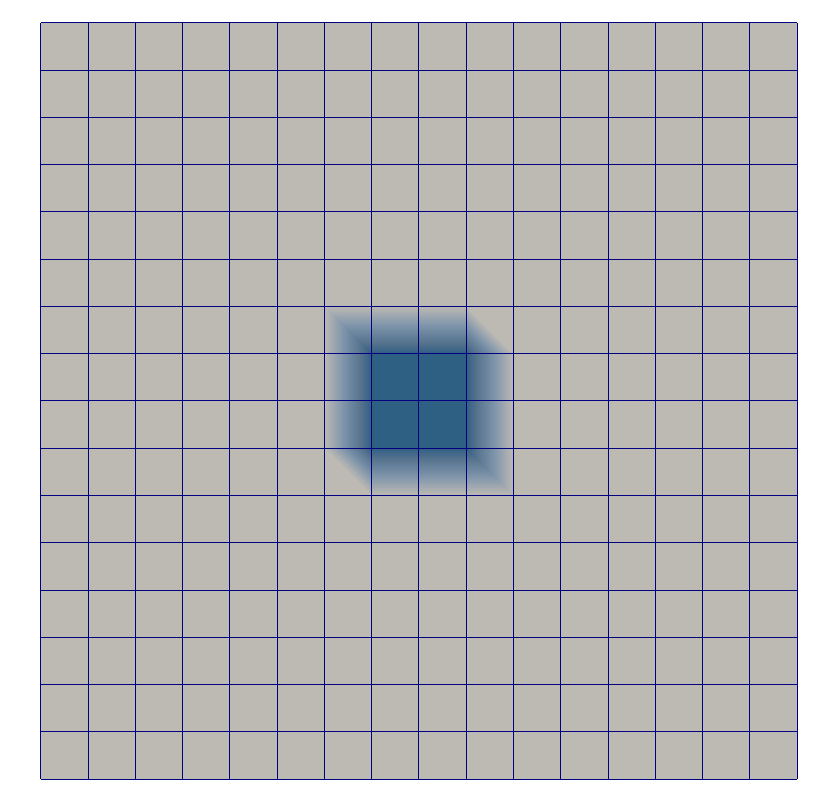
\includegraphics[width=4cm]{images/stokes_sphere2D/aspect_FS_gr/C1_gr3}
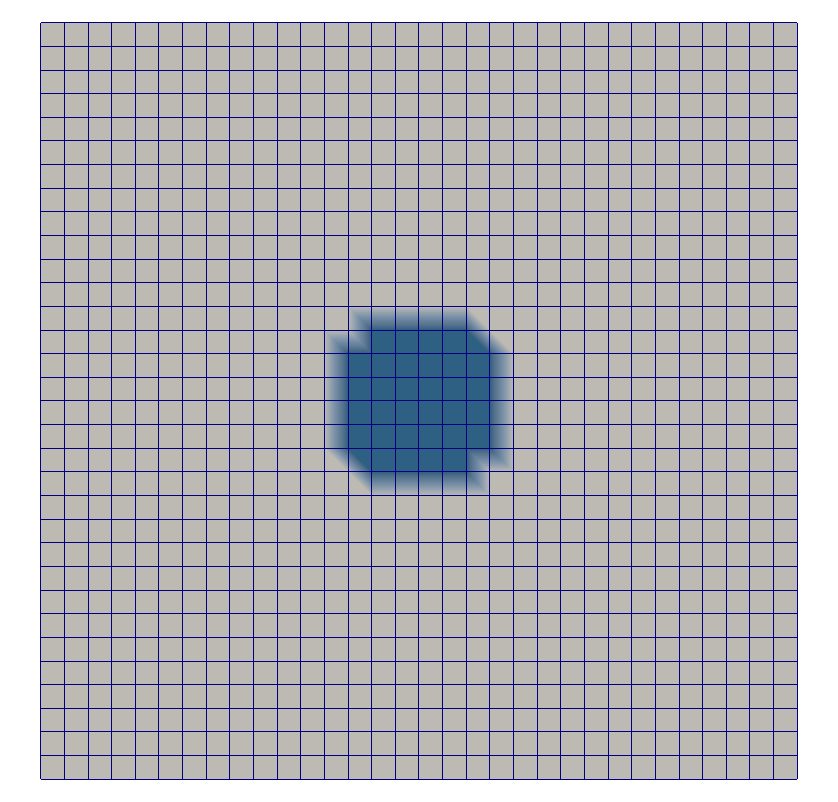
\includegraphics[width=4cm]{images/stokes_sphere2D/aspect_FS_gr/C1_gr4}
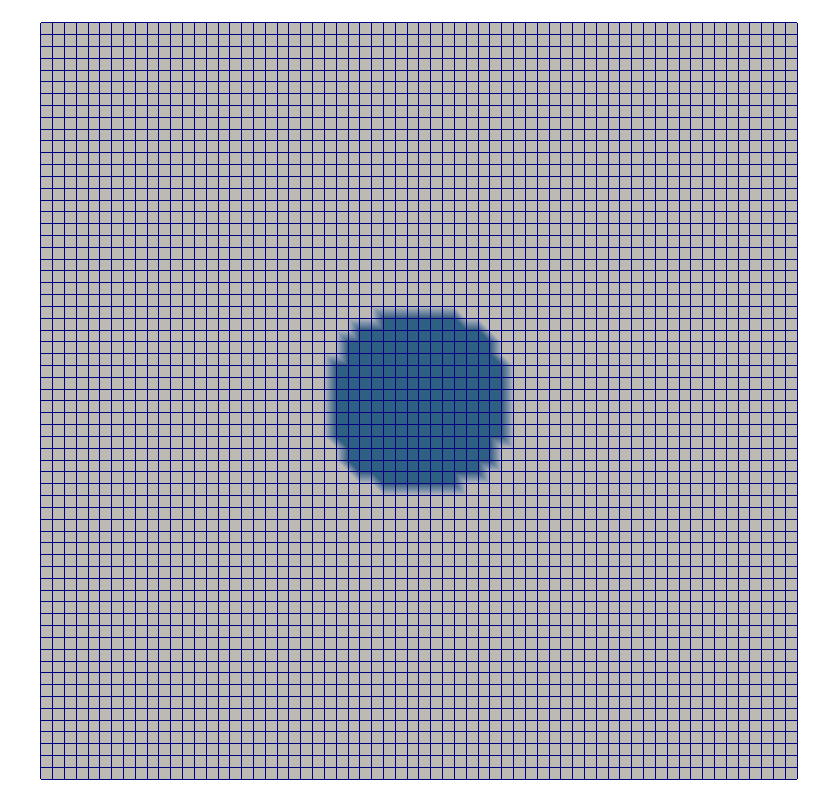
\includegraphics[width=4cm]{images/stokes_sphere2D/aspect_FS_gr/C1_gr5}
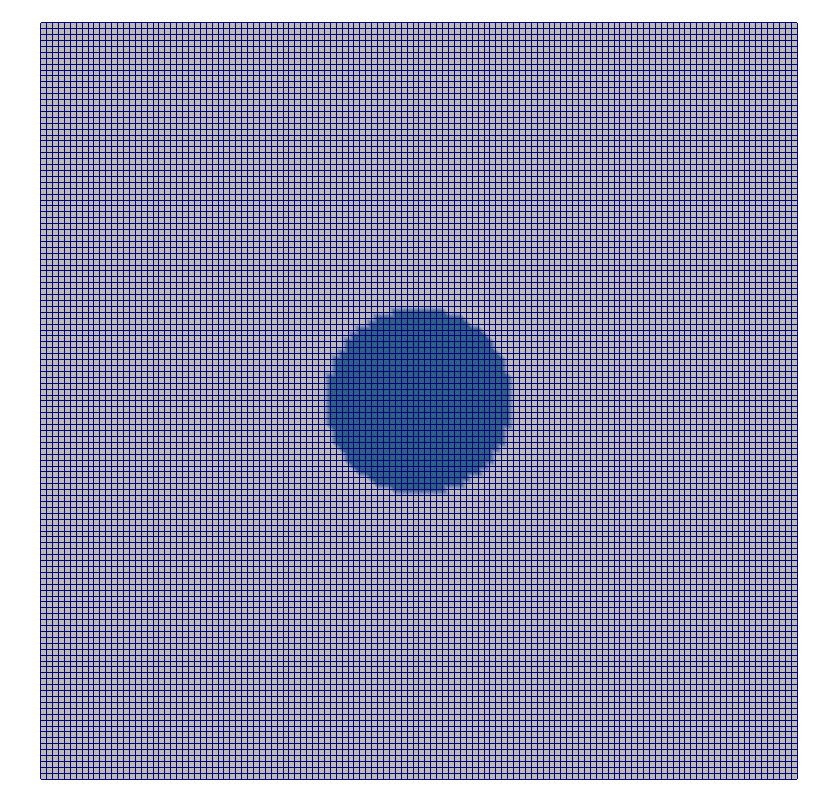
\includegraphics[width=4cm]{images/stokes_sphere2D/aspect_FS_gr/C1_gr6}
\end{center}


\begin{center}
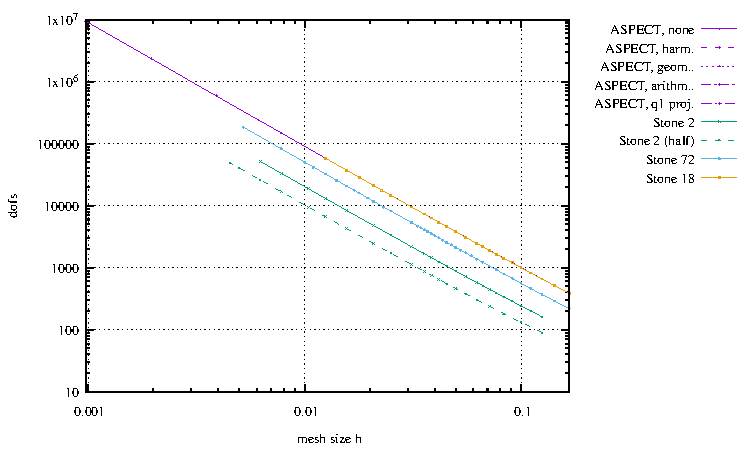
\includegraphics[width=7cm]{images/stokes_sphere2D/dofs}
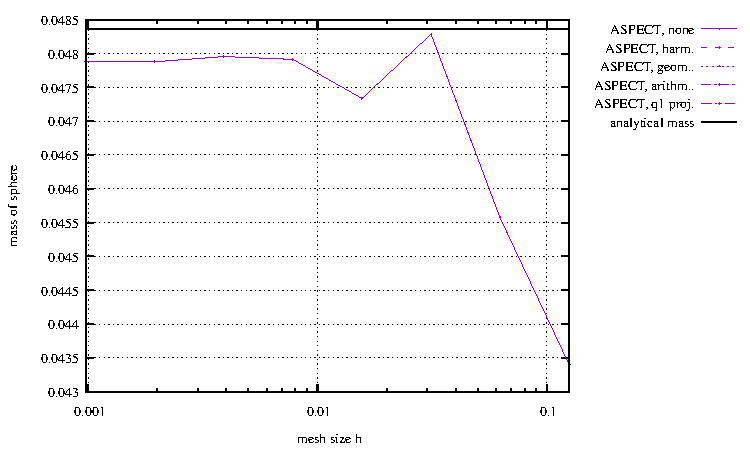
\includegraphics[width=7cm]{images/stokes_sphere2D/mass_sphere}\\
{\captionfont Left: total number of dofs in the Stokes problem; Right: mass of composition 1 
as measured in \aspect.}
\end{center}

The total mass of the system is 
\begin{eqnarray}
M 
&=& (L_xL_y-\pi R^2)\rho_{fluid} + \pi R^2 \rho_{sphere} \\
&=& (L_xL_y-\pi R^2)\rho_{fluid} + \pi R^2 (\rho_{fluid} + \delta\rho)\\
&=& L_xL_y \rho_{fluid} + \pi R^2 \delta\rho\\
&=& 1 + \pi \cdot 0.123456789^2 \cdot 0.01\\
&\simeq& 1.00047882831
\end{eqnarray}

The Stokes velocity can be obtained as follows: on p61 of Landau \& Lifschitz, it is reported that the drag force 
on a disk moving in its plane is $F=32\eta_f R \upnu_s /3$. The buoyancy force is $F=\pi R^2 \delta \rho g$, so the 
velocity is then 
\[
\upnu_s = \frac{3 \pi}{32} \frac{\delta \rho}{\eta_f} R g \simeq 0.00036361025
\]
Given the dimensions, this is obviously given per meter of the infinite cylinder.
This is substantially smaller than what we recover, so I keep the 3D velocity as reference for now.


In a second time, we make use of the mesh refinement capabilities of the code, as shown here:
\begin{center}
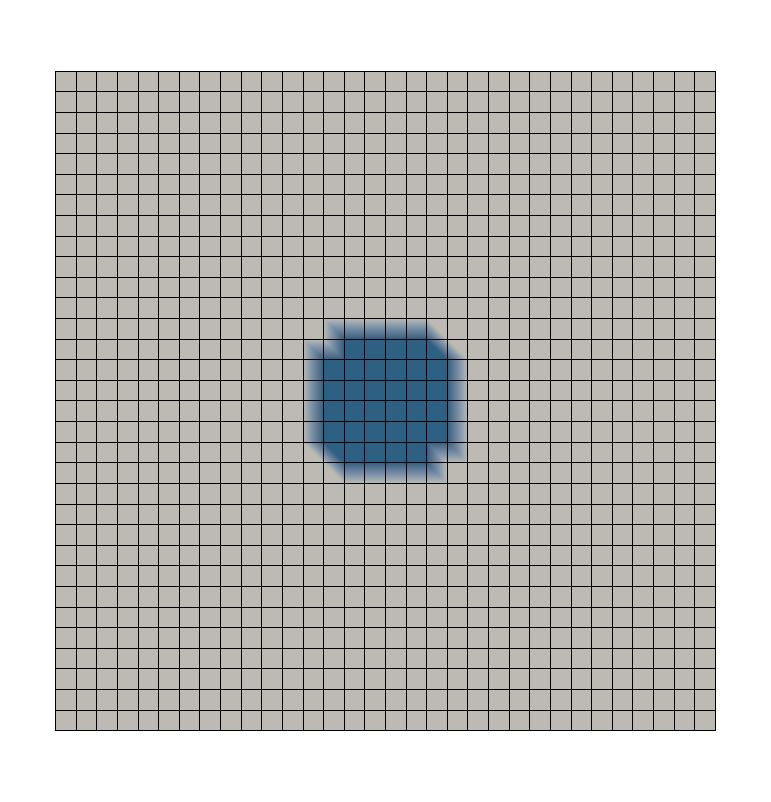
\includegraphics[width=4cm]{images/stokes_sphere2D/aspect_FS_amr/C1_0}
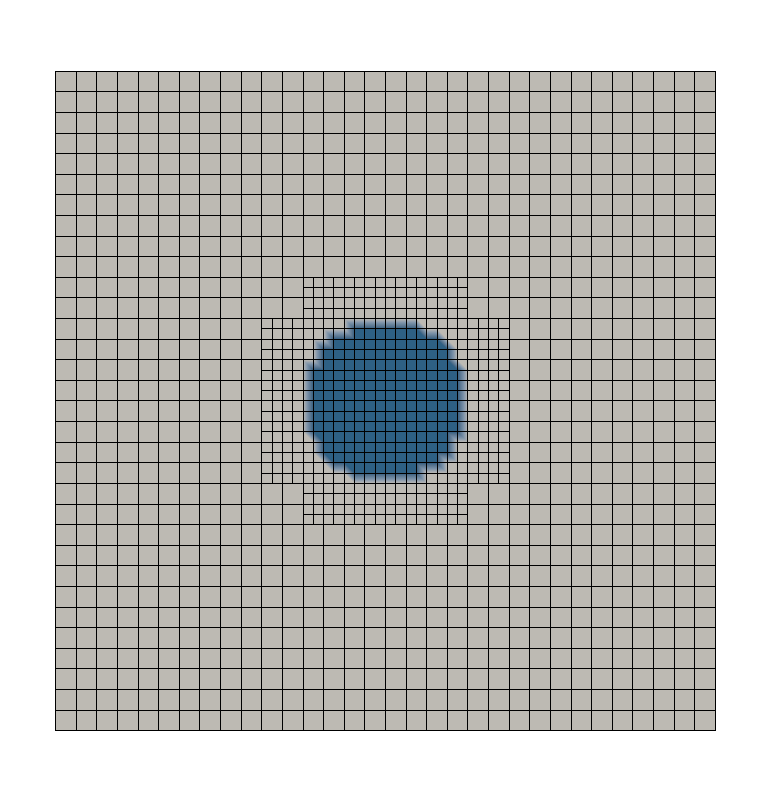
\includegraphics[width=4cm]{images/stokes_sphere2D/aspect_FS_amr/C1_1}
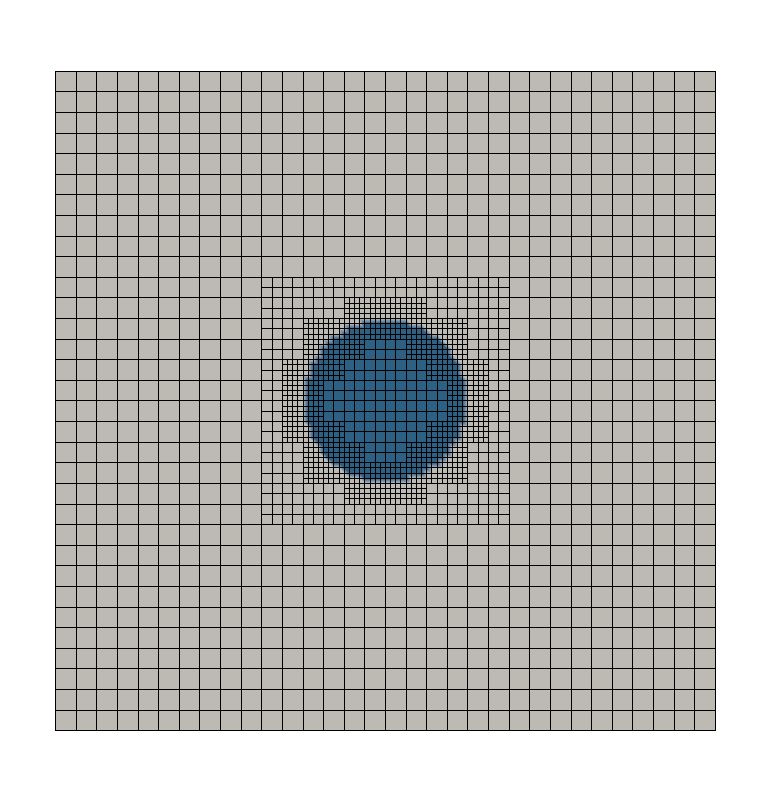
\includegraphics[width=4cm]{images/stokes_sphere2D/aspect_FS_amr/C1_2}
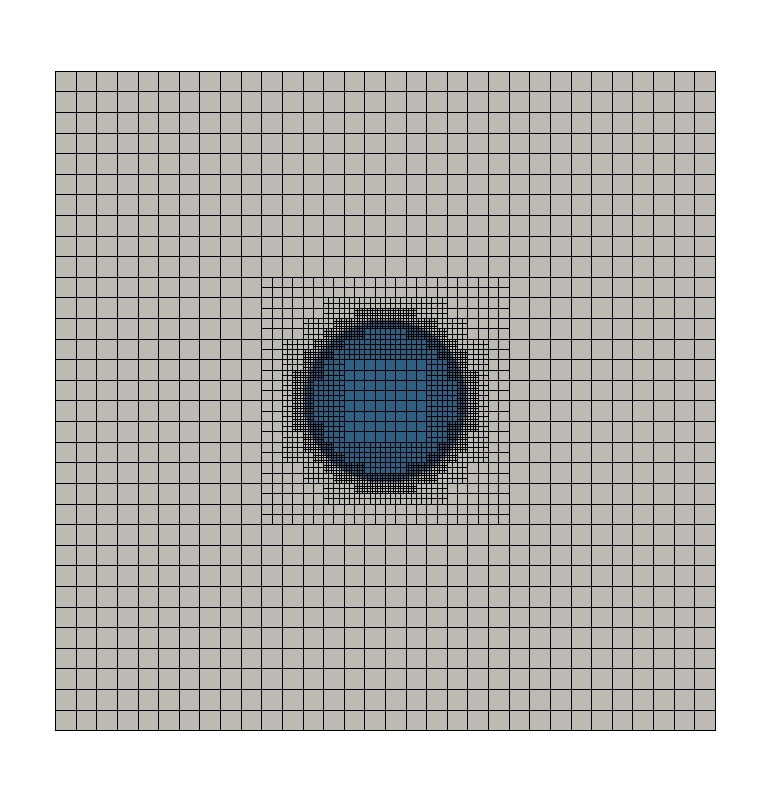
\includegraphics[width=4cm]{images/stokes_sphere2D/aspect_FS_amr/C1_3}\\
{\captionfont Octree-based \aspect meshes. The background mesh is $16^3$ and refinement is allowed to take place 4 times.
Note that a special output is automatically generated in the code which subdivides all elements in 8 for 
visualisation purposes only. Initial refinements 0,1,2,3,4.}
\end{center}
This corresponds to 
\begin{verbatim}
subsection Mesh refinement
set Initial adaptive refinement = 0 -> 9 
set Initial global refinement = 4 
set Refinement fraction = 0.9 
set Coarsening fraction = 0 
set Strategy = composition
end
\end{verbatim}

\newpage
%.................................................................................
\paragraph{FS results}

\begin{center}
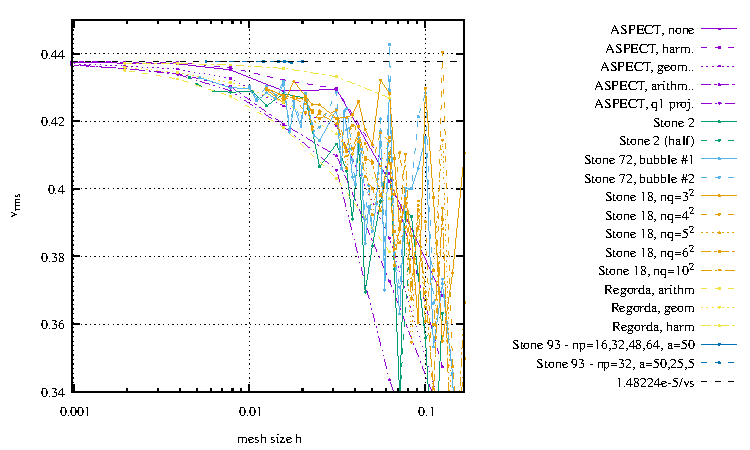
\includegraphics[width=7cm]{images/stokes_sphere2D/vrms_FS}
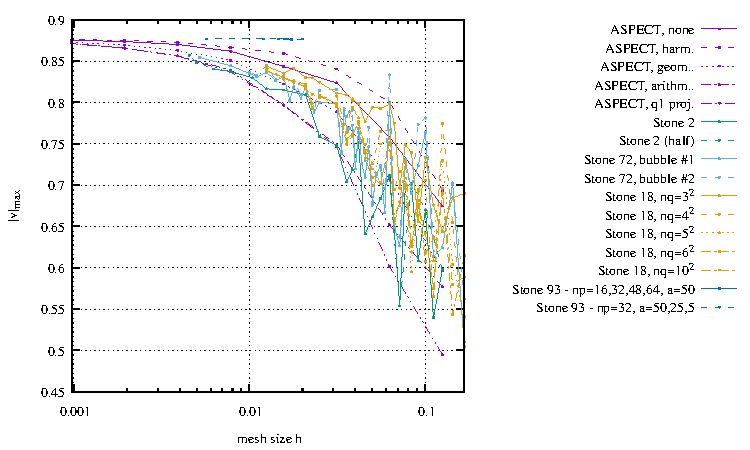
\includegraphics[width=7cm]{images/stokes_sphere2D/max_vel_FS}\\
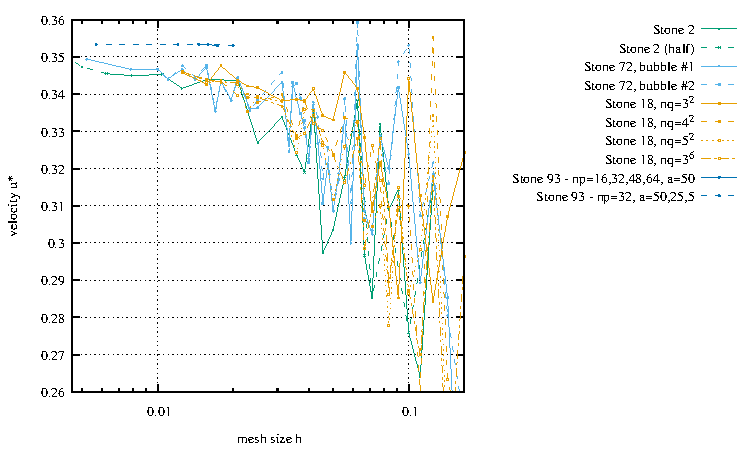
\includegraphics[width=7cm]{images/stokes_sphere2D/max_u_FS}
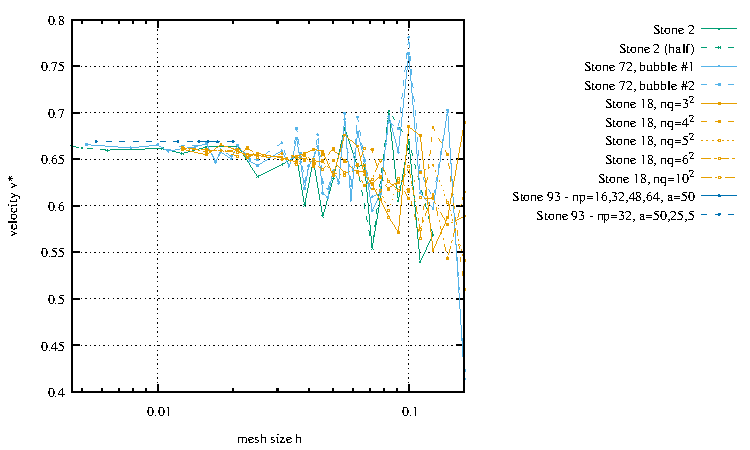
\includegraphics[width=7cm]{images/stokes_sphere2D/max_v_FS}\\
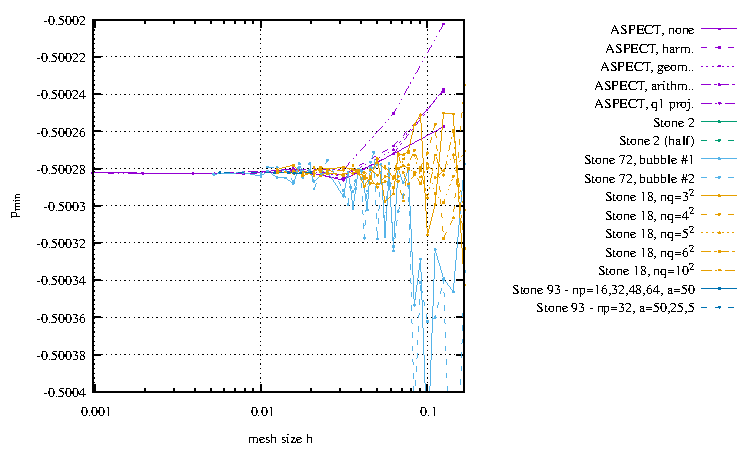
\includegraphics[width=7cm]{images/stokes_sphere2D/pressure_min_FS}
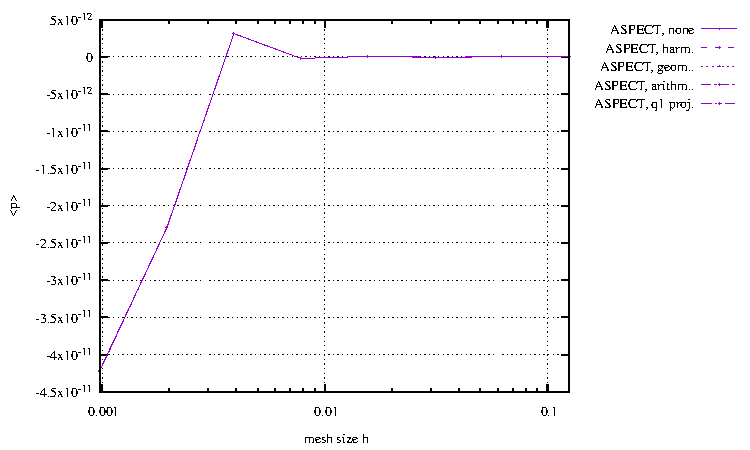
\includegraphics[width=7cm]{images/stokes_sphere2D/pressure_mean_FS}\\
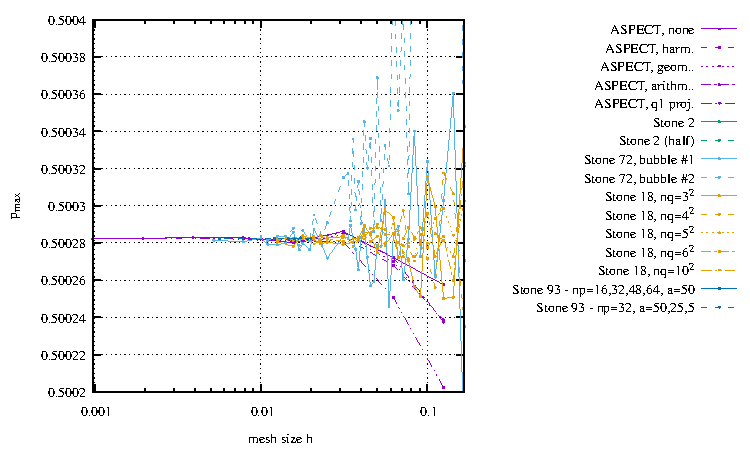
\includegraphics[width=7cm]{images/stokes_sphere2D/pressure_max_FS}
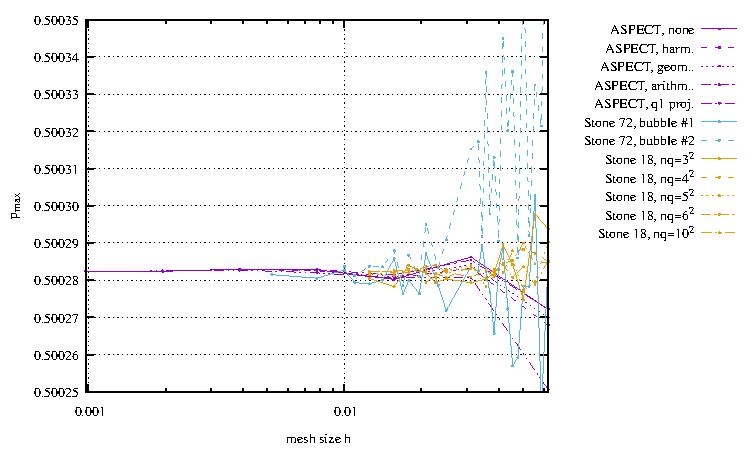
\includegraphics[width=7cm]{images/stokes_sphere2D/pressure_max_FS_zoom}\\
{\captionfont Measurements obtained with \aspect for various averaging schemes and with different stones.}
\end{center}

\begin{center}
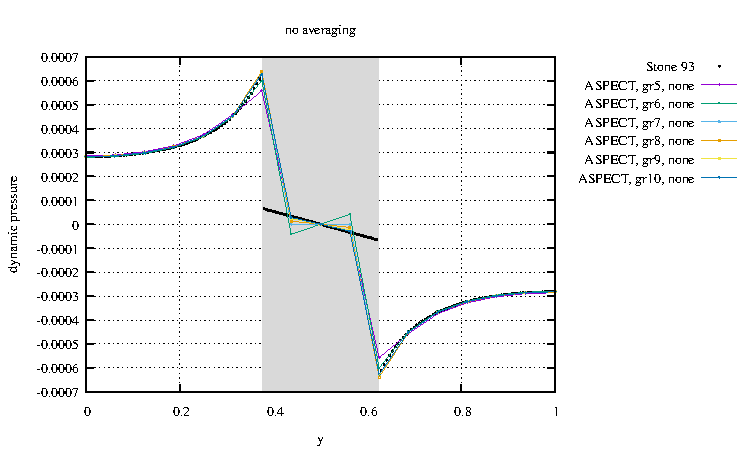
\includegraphics[width=5.7cm]{images/stokes_sphere2D/pressure_profile_none_FS.pdf}
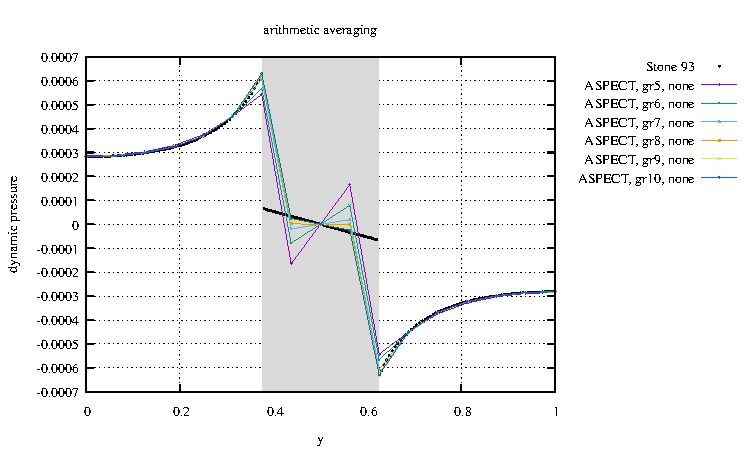
\includegraphics[width=5.7cm]{images/stokes_sphere2D/pressure_profile_arithmetic_FS.pdf}
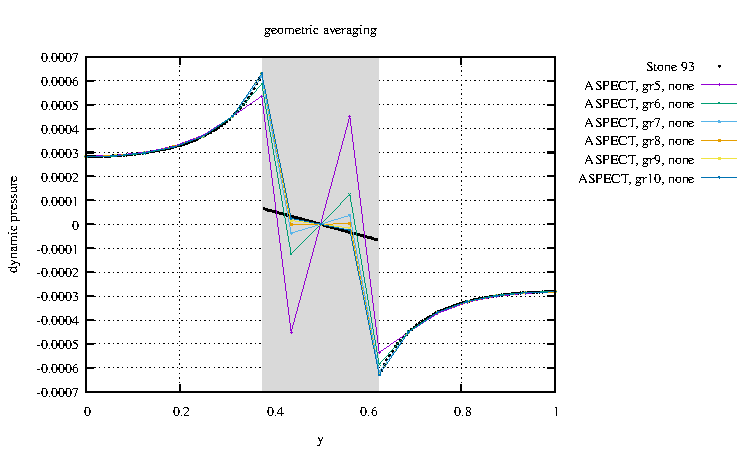
\includegraphics[width=5.7cm]{images/stokes_sphere2D/pressure_profile_geometric_FS.pdf}\\
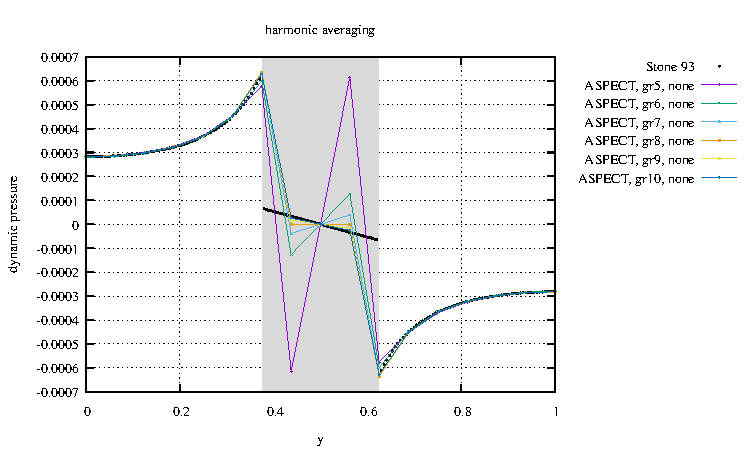
\includegraphics[width=5.7cm]{images/stokes_sphere2D/pressure_profile_harmonic_FS.pdf}
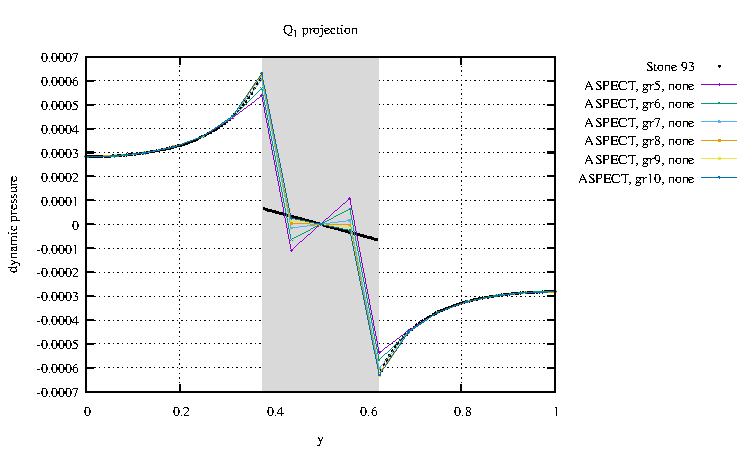
\includegraphics[width=5.7cm]{images/stokes_sphere2D/pressure_profile_q1_FS.pdf}
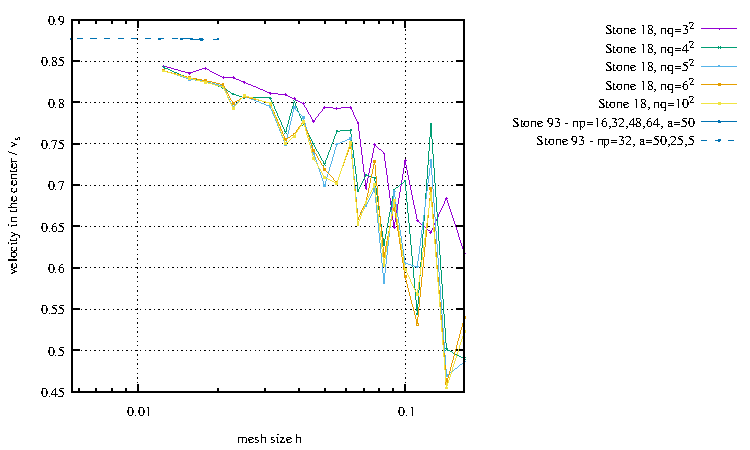
\includegraphics[width=5.7cm]{images/stokes_sphere2D/center_velocity_FS}
\end{center}




\newpage
%.................................................................................
\paragraph{NS results}

\begin{center}
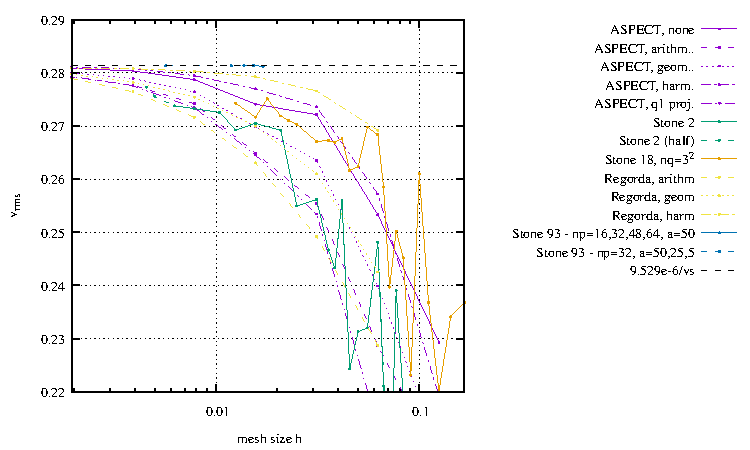
\includegraphics[width=7cm]{images/stokes_sphere2D/vrms_NS}
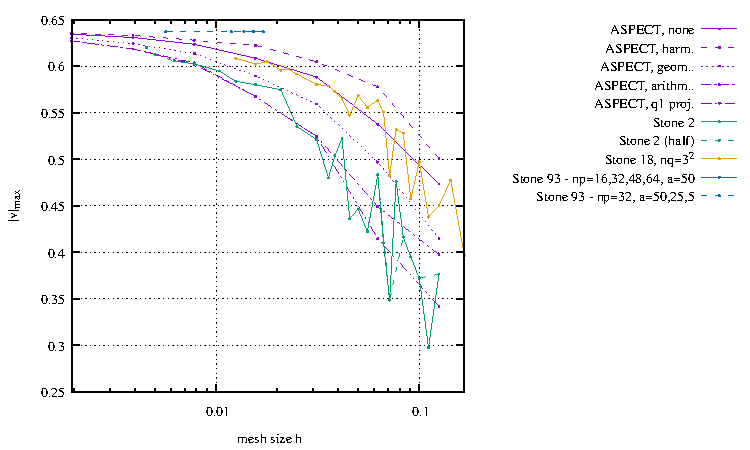
\includegraphics[width=7cm]{images/stokes_sphere2D/max_vel_NS}\\
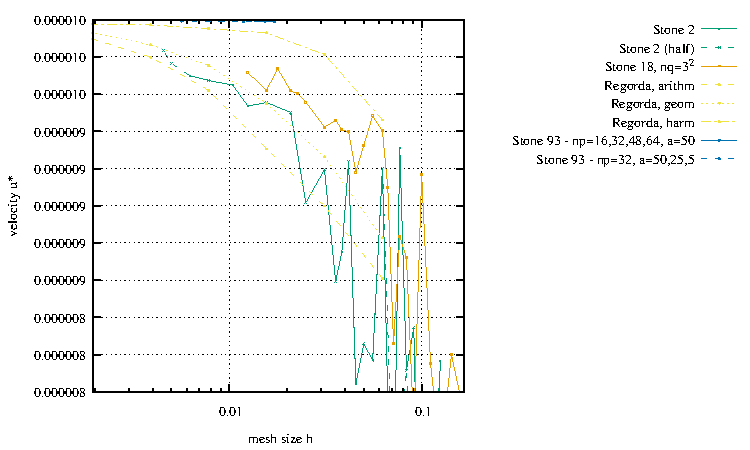
\includegraphics[width=7cm]{images/stokes_sphere2D/max_u_NS}
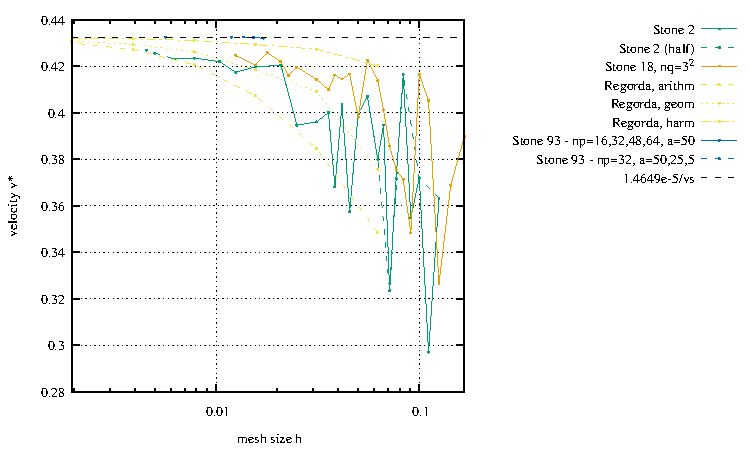
\includegraphics[width=7cm]{images/stokes_sphere2D/max_v_NS}\\
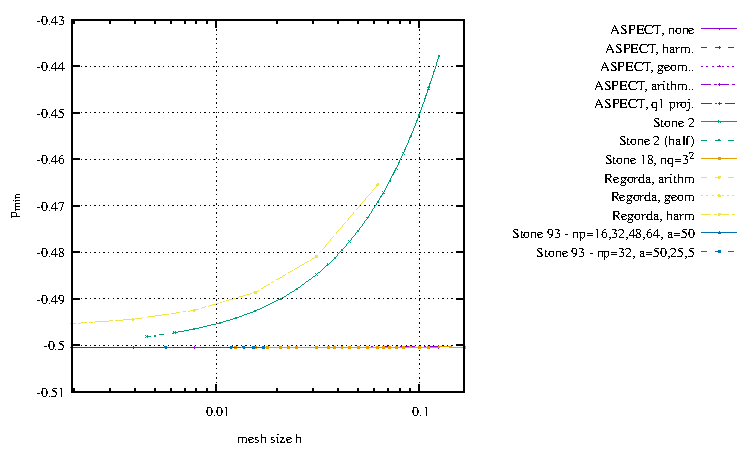
\includegraphics[width=7cm]{images/stokes_sphere2D/pressure_min_NS}
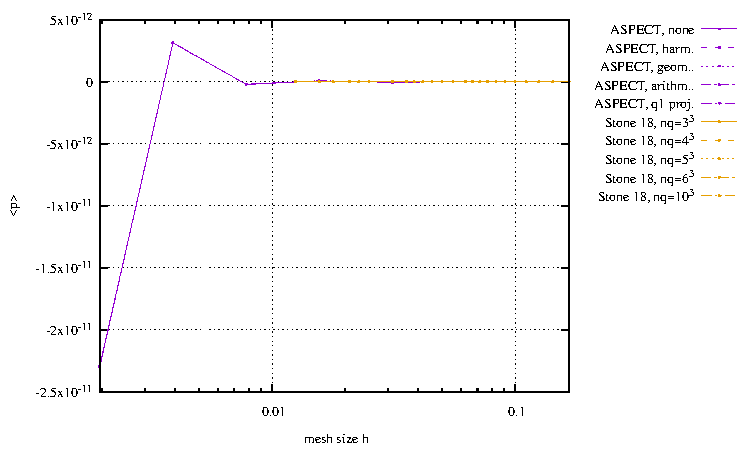
\includegraphics[width=7cm]{images/stokes_sphere2D/pressure_mean_NS}
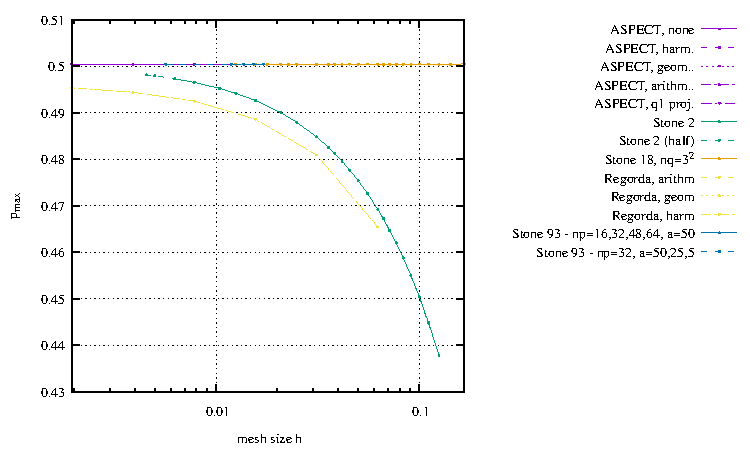
\includegraphics[width=7cm]{images/stokes_sphere2D/pressure_max_NS}\\
{\captionfont Measurements obtained with \aspect for various averaging schemes and with different stones.}
\end{center}


I have also retrieved the pressure at 16 equidistant locations on the $x=0.5$ line
for all five averagings. Because the signal is dominated by the lithostatic 
pressure I have subtracted it from the data, so that I hereunder plot the 
dynamic pressure as a function of the $y$ coordinate:

\begin{center}
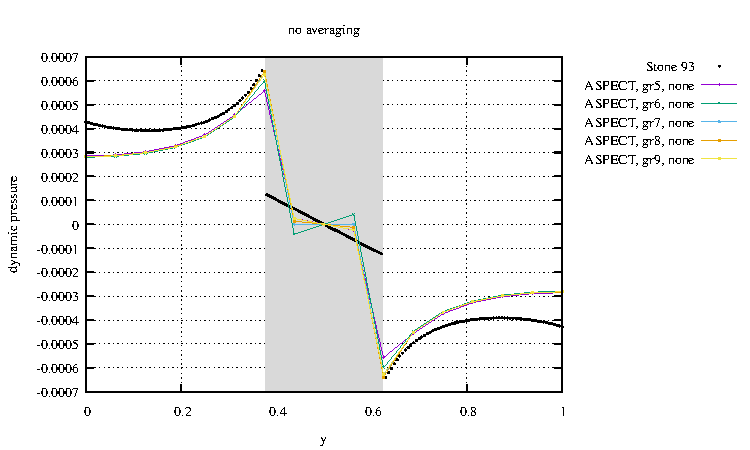
\includegraphics[width=5.7cm]{images/stokes_sphere2D/pressure_profile_none_NS.pdf}
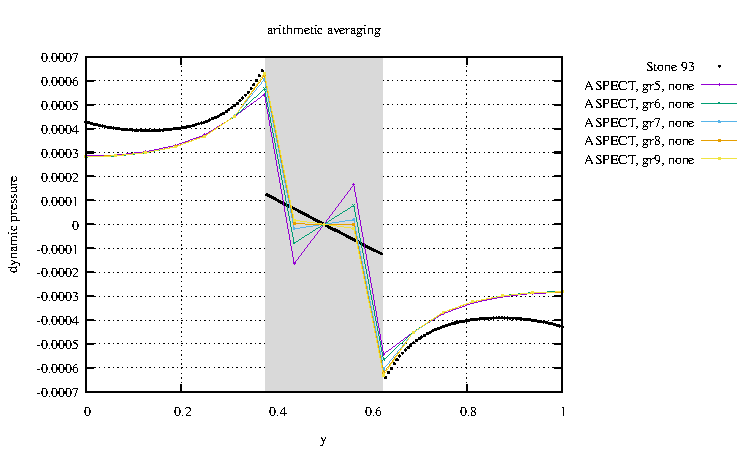
\includegraphics[width=5.7cm]{images/stokes_sphere2D/pressure_profile_arithmetic_NS.pdf}
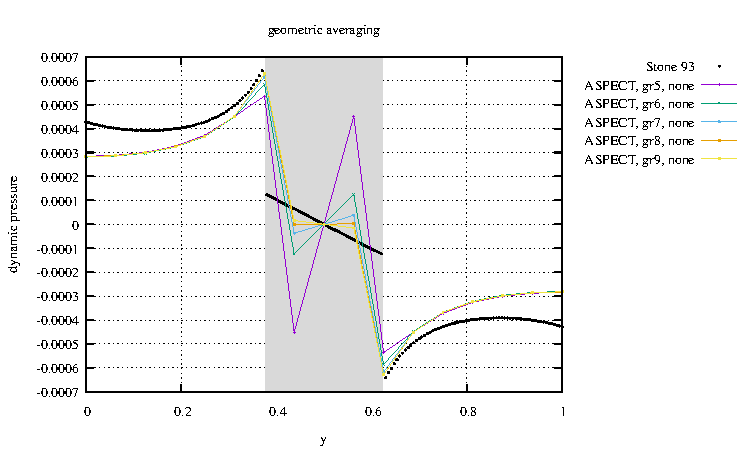
\includegraphics[width=5.7cm]{images/stokes_sphere2D/pressure_profile_geometric_NS.pdf}\\
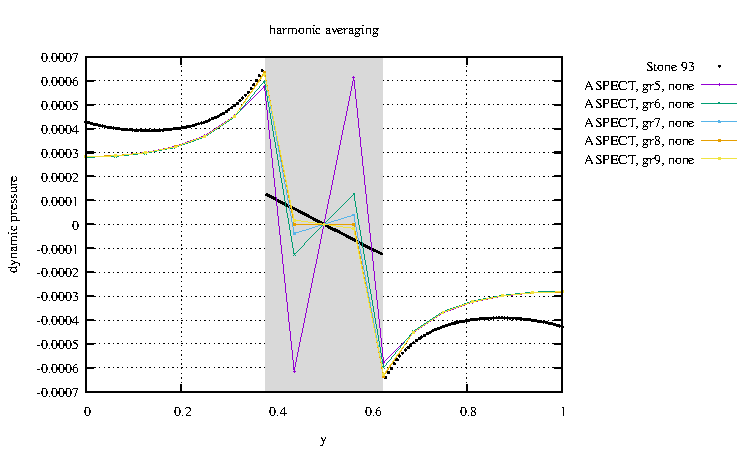
\includegraphics[width=5.7cm]{images/stokes_sphere2D/pressure_profile_harmonic_NS.pdf}
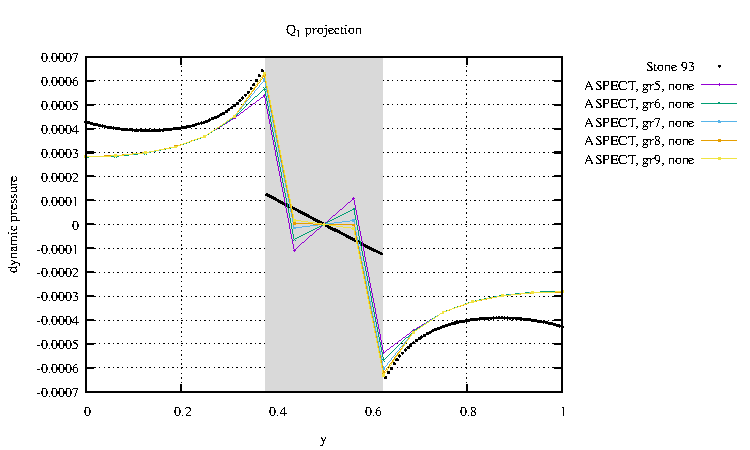
\includegraphics[width=5.7cm]{images/stokes_sphere2D/pressure_profile_q1_NS.pdf}\\
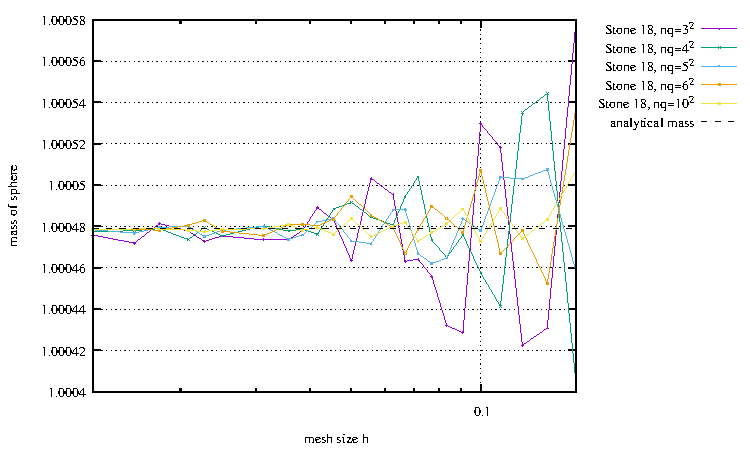
\includegraphics[width=5.7cm]{images/stokes_sphere2D/mass_total}
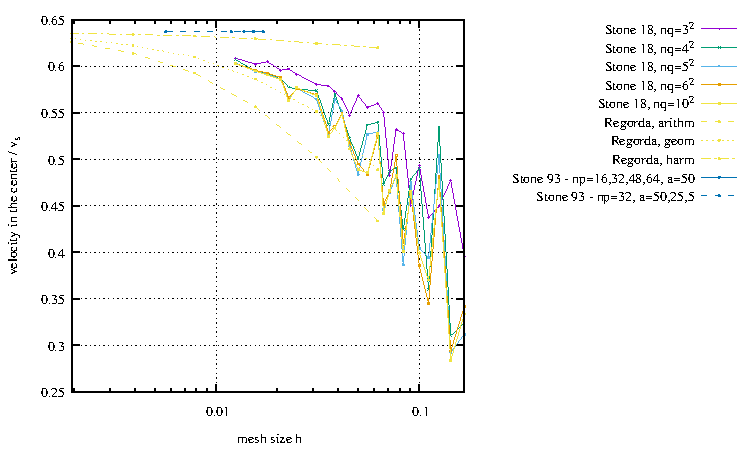
\includegraphics[width=5.7cm]{images/stokes_sphere2D/center_velocity_NS}
\end{center}


\newpage
%.................................................................................
\paragraph{OT results}

\begin{center}
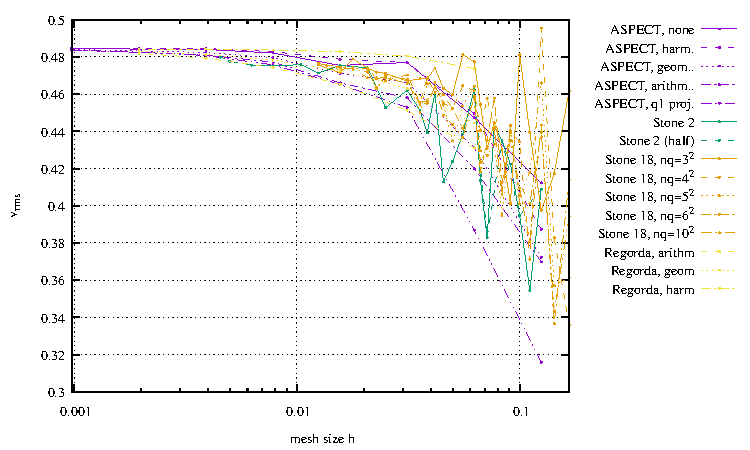
\includegraphics[width=7cm]{images/stokes_sphere2D/vrms_OT}
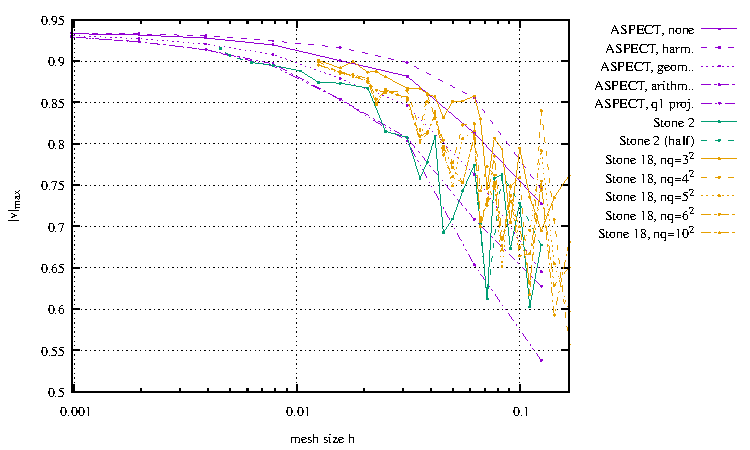
\includegraphics[width=7cm]{images/stokes_sphere2D/max_vel_OT}\\
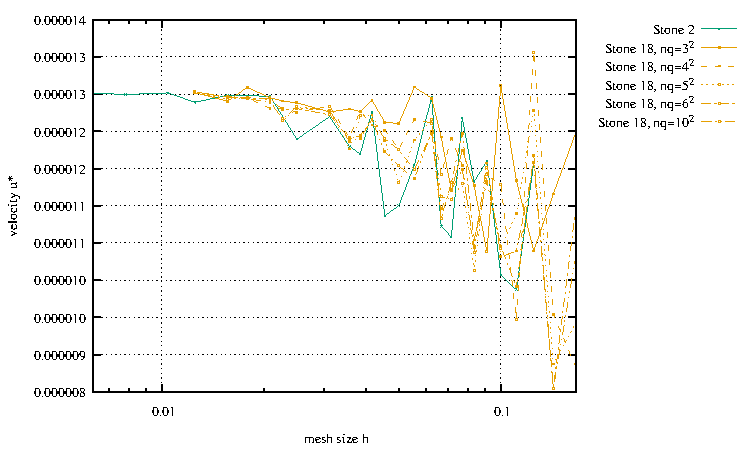
\includegraphics[width=7cm]{images/stokes_sphere2D/max_u_OT}
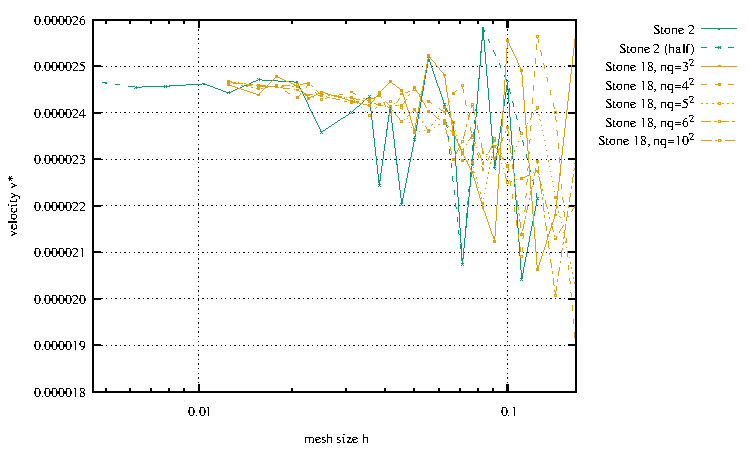
\includegraphics[width=7cm]{images/stokes_sphere2D/max_v_OT}\\
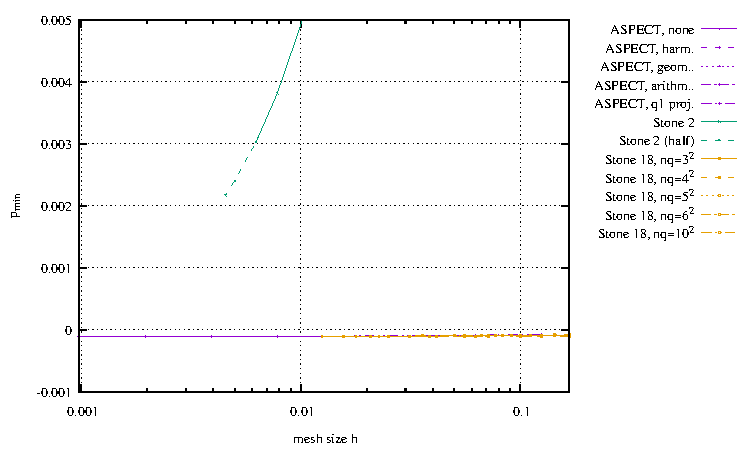
\includegraphics[width=7cm]{images/stokes_sphere2D/pressure_min_OT}
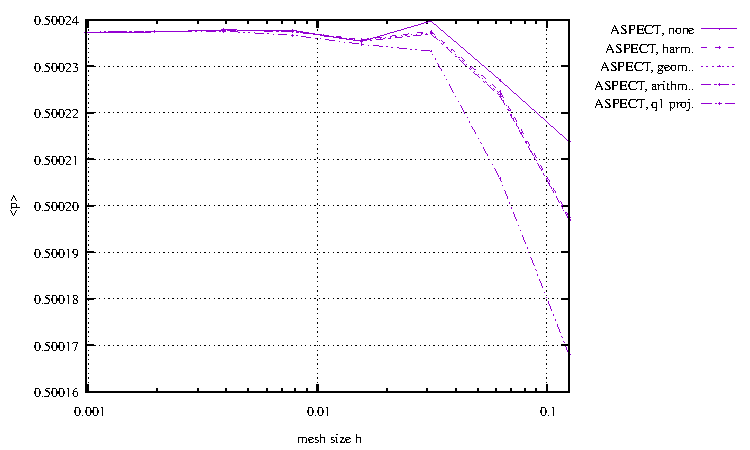
\includegraphics[width=7cm]{images/stokes_sphere2D/pressure_mean_OT}\\
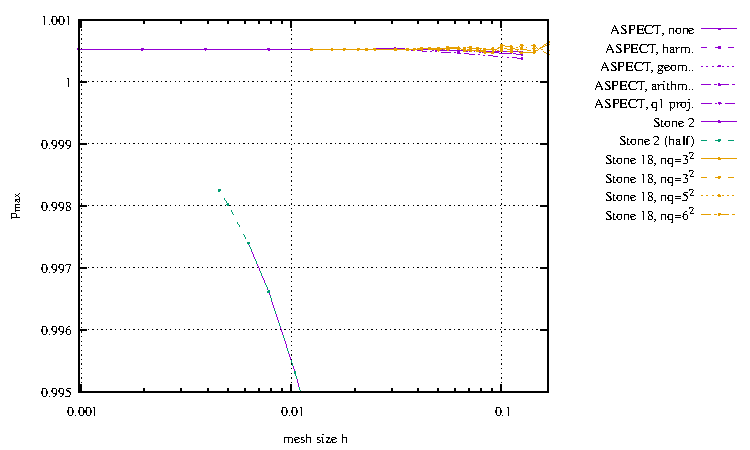
\includegraphics[width=7cm]{images/stokes_sphere2D/pressure_max_OT}
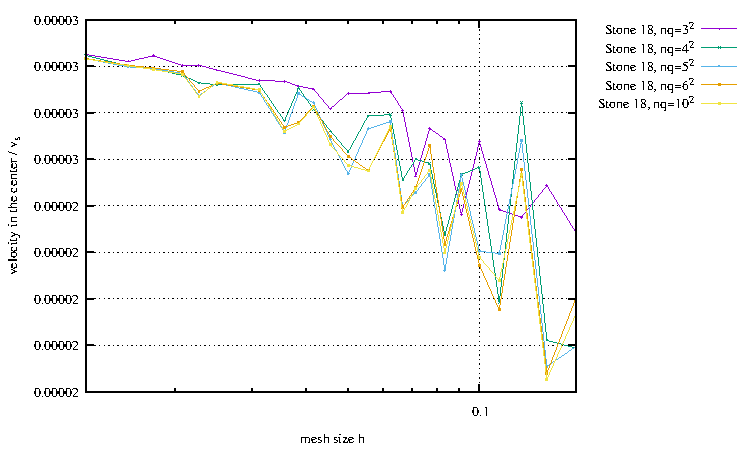
\includegraphics[width=7cm]{images/stokes_sphere2D/center_velocity_OT}\\
{\captionfont Measurements obtained with \aspect for various averaging schemes and with different stones.}
\end{center}

\begin{center}
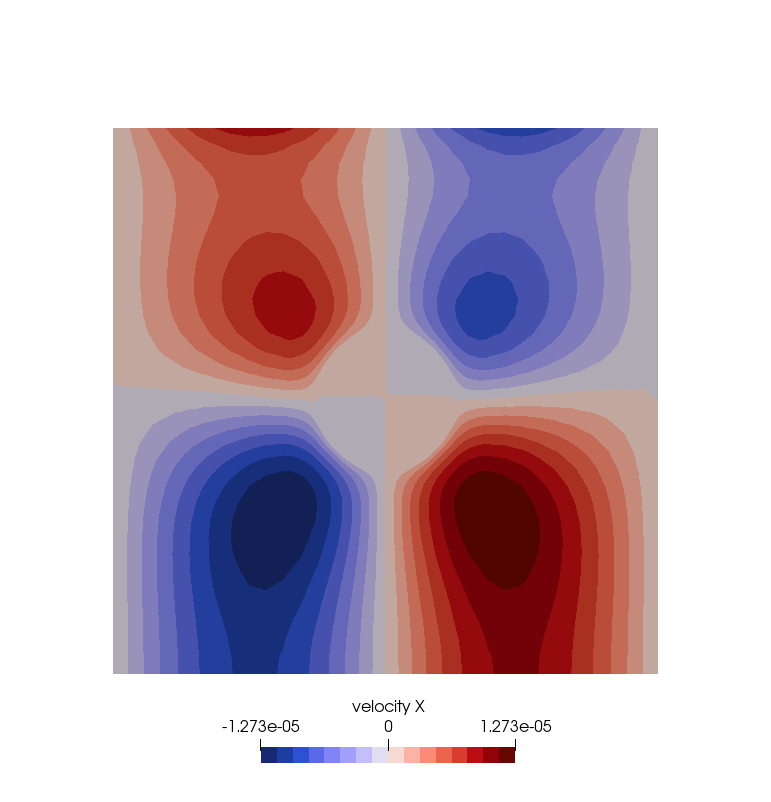
\includegraphics[width=5cm]{images/stokes_sphere2D/aspect_OT_amr/u}
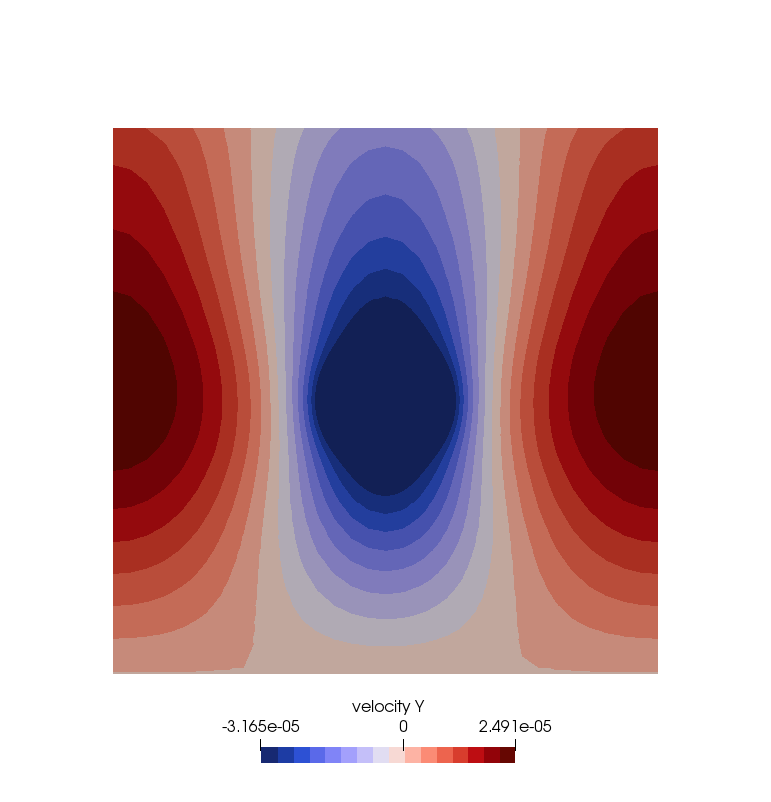
\includegraphics[width=5cm]{images/stokes_sphere2D/aspect_OT_amr/v}
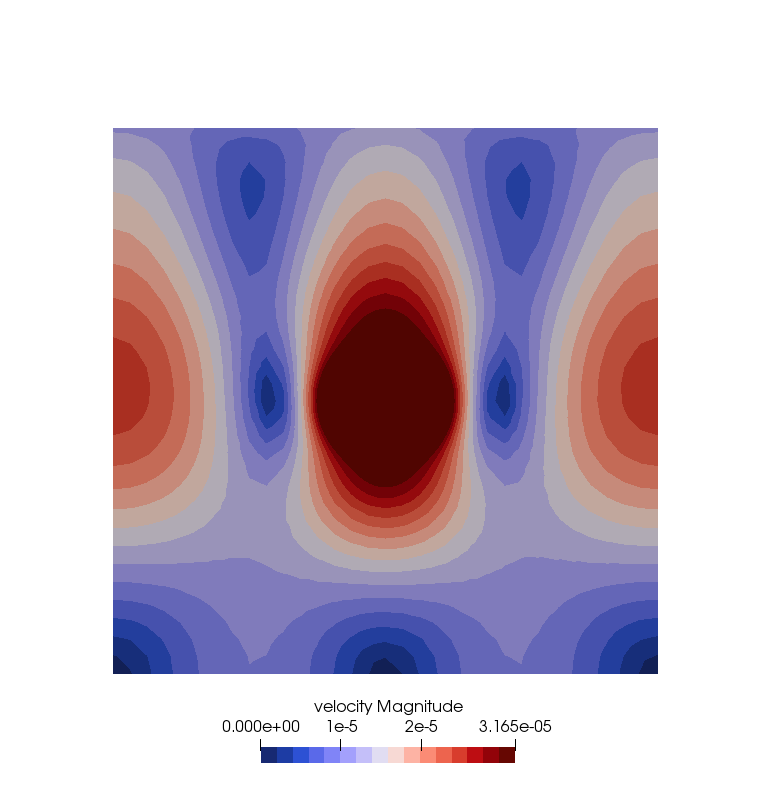
\includegraphics[width=5cm]{images/stokes_sphere2D/aspect_OT_amr/vel}
\end{center}



\newpage
%.................................................................................
\paragraph{BO results}.



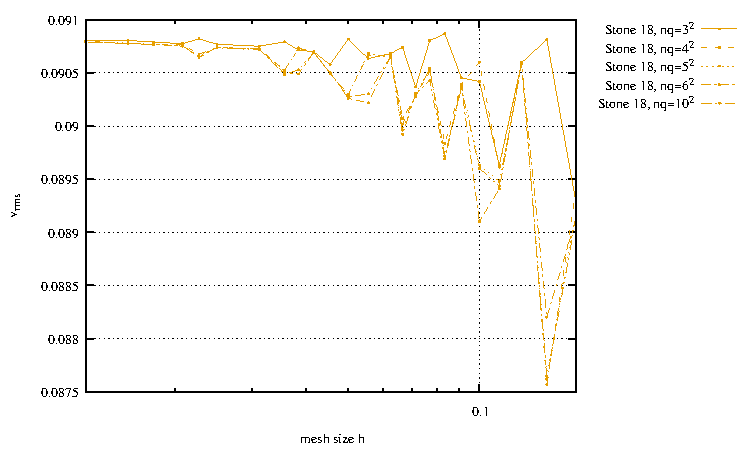
\includegraphics[width=7cm]{images/stokes_sphere2D/vrms_BO}
\includegraphics[width=7cm]{images/stokes_sphere2D/center_velocity_BO}

\includegraphics[width=5.7cm]{images/stokes_sphere2D/stone18_BO/u}
\includegraphics[width=5.7cm]{images/stokes_sphere2D/stone18_BO/v}
\includegraphics[width=5.7cm]{images/stokes_sphere2D/stone18_BO/vel}\\
\includegraphics[width=5.7cm]{images/stokes_sphere2D/stone18_BO/press}
\includegraphics[width=5.7cm]{images/stokes_sphere2D/stone18_BO/exx}
\includegraphics[width=5.7cm]{images/stokes_sphere2D/stone18_BO/exy}




